% Fig. 2 -- Software architecture: the research pipeline and the BeeMove
% application share one Python package, so the code evaluated in the paper is
% the code users run.
\documentclass[tikz,border=2pt]{standalone}
\usepackage[T1]{fontenc}
\usepackage[scaled=0.92]{helvet}
\renewcommand{\familydefault}{\sfdefault}
\usetikzlibrary{arrows.meta,positioning,fit,backgrounds,calc,shapes.geometric}

\begin{document}
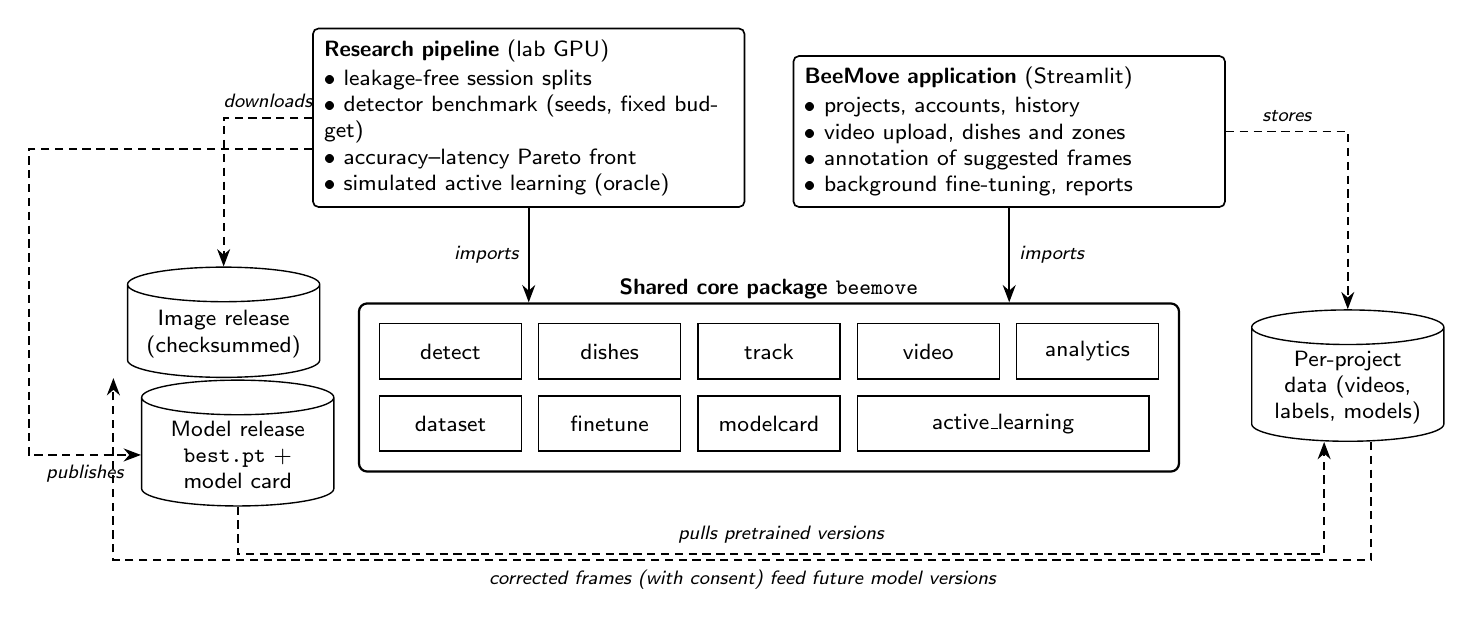
\begin{tikzpicture}[
  font=\footnotesize,
  >={Stealth[length=2.2mm]},
  mod/.style={draw, align=center, minimum height=7mm, text width=17mm,
              inner sep=1.5pt, line width=0.5pt, fill=white},
  comp/.style={draw, rounded corners=2pt, align=left, text width=52mm,
               inner sep=4pt, line width=0.6pt},
  store/.style={draw, cylinder, shape border rotate=90, aspect=0.18,
                align=center, text width=23mm, minimum height=14mm,
                inner sep=2pt, line width=0.5pt},
  flow/.style={->, line width=0.7pt},
  dflow/.style={->, line width=0.7pt, densely dashed},
  lbl/.style={font=\scriptsize\itshape, align=center},
]

% ------------------------------------------------------------ shared package
\node[mod] (m1) {detect};
\node[mod, right=2mm of m1] (m2) {dishes};
\node[mod, right=2mm of m2] (m3) {track};
\node[mod, right=2mm of m3] (m4) {video};
\node[mod, right=2mm of m4] (m5) {analytics};
\node[mod, below=2mm of m1] (m6) {dataset};
\node[mod, right=2mm of m6] (m7) {finetune};
\node[mod, right=2mm of m7] (m8) {modelcard};
\node[mod, right=2mm of m8, text width=36mm] (m9) {active\_learning};
\node[draw, line width=0.8pt, rounded corners=3pt, inner sep=2.5mm,
      fit=(m1)(m5)(m6)(m9)] (core) {};
\node[font=\footnotesize\bfseries, anchor=south, fill=white, inner sep=1pt]
     at (core.north) {Shared core package \texttt{beemove}};

% ------------------------------------------------------------ two consumers
\node[comp, anchor=south east] (research) at ($(core.north)+(-3mm,12mm)$) {%
  \textbf{Research pipeline} (lab GPU)\\[1pt]
  \textbullet\ leakage-free session splits\\
  \textbullet\ detector benchmark (seeds, fixed budget)\\
  \textbullet\ accuracy--latency Pareto front\\
  \textbullet\ simulated active learning (oracle)};
\node[comp, anchor=south west] (app) at ($(core.north)+(3mm,12mm)$) {%
  \textbf{BeeMove application} (Streamlit)\\[1pt]
  \textbullet\ projects, accounts, history\\
  \textbullet\ video upload, dishes and zones\\
  \textbullet\ annotation of suggested frames\\
  \textbullet\ background fine-tuning, reports};

\draw[flow] (research.south) -- node[lbl, left] {imports} (research.south |- core.north);
\draw[flow] (app.south) -- node[lbl, right] {imports} (app.south |- core.north);

% ------------------------------------------------------------ artefacts
\node[store, left=9mm of core.north west, anchor=north east, yshift=4mm] (data) {Image release\\(checksummed)};
\node[store, left=9mm of core.south west, anchor=south east, yshift=-4mm] (models) {Model release\\\texttt{best.pt} +\\model card};
\node[store, right=9mm of core.east, anchor=west] (proj) {Per-project\\data (videos,\\labels, models)};

\draw[dflow] (research.west) -| node[lbl, pos=0.25, above] {downloads} (data.north);
\draw[dflow] (research.west) ++(0,-4mm) -- ++(-36mm,0) |- node[lbl, pos=0.75, below] {publishes} (models.west);
\draw[dflow] (app.east) -| node[lbl, pos=0.25, above] {stores} (proj.north);
\draw[dflow] (models.south) -- ++(0,-6mm) -| node[lbl, pos=0.25, above] {pulls pretrained versions} ([xshift=-3mm]proj.south);
\draw[dflow] ([xshift=3mm]proj.south) -- ++(0,-15mm) -| node[lbl, pos=0.25, below] {corrected frames (with consent) feed future model versions} ([xshift=-14mm]data.south);

\end{tikzpicture}
\end{document}
